\documentclass{article}
\usepackage{amsthm}
\usepackage{amsmath}
\usepackage{graphicx}
\usepackage{multirow}
\usepackage{tikz}
\usepackage{wasysym}
\newtheorem{problem}{Problem}

\begin{document}
\title{Playing Games}
\author{Henry Z. Lo}
\maketitle

\section{Games}
We consider writing AI to play games with the following properties:
\begin{itemize}
\item Two players.
\item Determinism: no chance is involved; game state based purely on decisions made by players.
\item No hidden information: at any given time, both players have the same amount of knowledge.
\item Finite states: a limited number of possible game states.
\end{itemize}
By game state, we mean state of the board, which contains all the necessary information about the current game (along with whose turn it is).  Games which satisfy these properties include checkers, chess, tic-tac-toe, and nim.

\subsection{Game Trees}
Games satisfying these criteria can be represented completely using a game tree.  The tree is built as such:
\begin{itemize}
\item The root represents the current game state.
\item Every other node represents a possible future game state.
\item Each node has as its children all game states which can be reached in one move.
\end{itemize}
Thus, leaves of the tree signify ways in which the game can end.  Paths from root to leaf represent how the game can evolve.  As an example, consider the partial game tree for tic-tac-toe in Figure \ref{tree1}.

It is important to know what player is making the current move.  In the games mentioned here, each level corresponds to a different player.  However, note that the game tree can accommodate players taking multiple turns in a row, as long as we know who is in control of the board at what node.

\begin{figure}
\centering
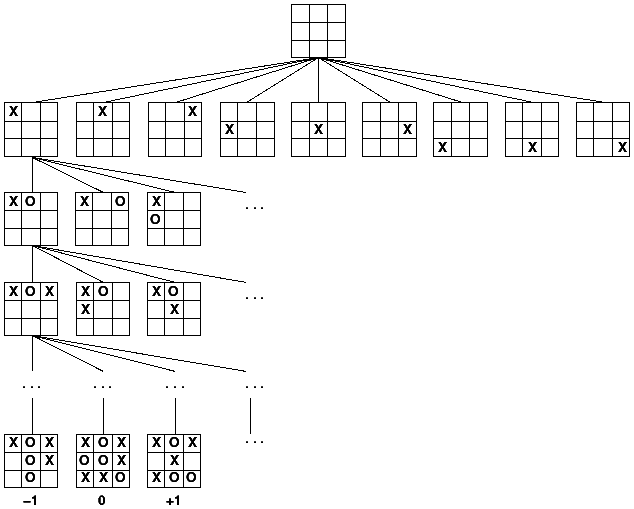
\includegraphics[width=1\textwidth]{img/game-tree.png}
\caption{Incomplete game tree for tic-tac-toe, in which $x$ goes first. \label{tree1}}
\end{figure}

\section{Game AI}
Given the entire game tree, it is possible to find the optimal sequence of moves, or paths, which solve the game.  How can we score the paths?

Consider if we were at the state $s$, which connects to several leaves.  We can score winning move as a +1, a losing move as a -1, and a draw as a 0.

What is the score of $s$?  It may not be so important if we were already at $s$, but it is relevant if getting to $s$ is an option.

\subsection{Minimax}
The score depends on the player.  We can assume that both us and our opponents will always take the best move available to them.  If the move from $s$ is ours, then we are in a pretty good position (we can get to 1).  If the move from $s$ is our opponents, then we will lose (opponent can get to -1).

The minimax algorithm uses this notion to recursively label nodes in a tree based on its children.  Labeling goes from leaf to root.  Once we get to the root, we can see which paths will definitely lead us to a win.  The minimax algorithm takes this path.  See Figure \ref{minimax}.

\begin{figure}
\centering
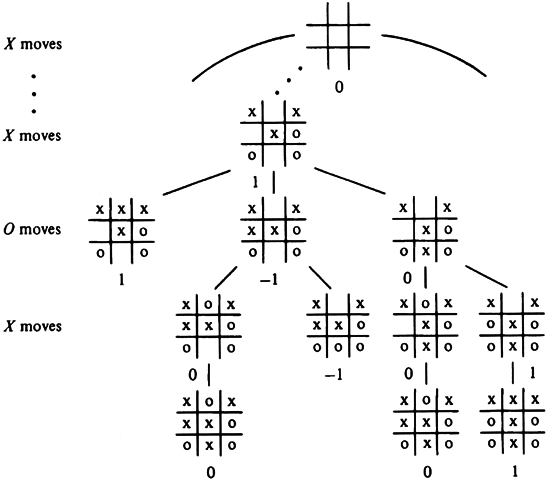
\includegraphics[width=1\textwidth]{img/minimax.png}
\caption{State scores +1 if it leads to a win for X, and -1 if it leads to a win for O. \label{minimax}}
\end{figure}

\begin{verbatim}
function minimax(node)
   if terminal node
      return 1 if win, 0 if draw, and -1 if loss
   if my turn
      bestValue = -infinity
      for each child of node
         bestValue = max(bestValue, minimax(child))
   else
      bestValue = infinity
      for each child of node
         bestValue = min(bestValue, minimax(child))      
   return bestValue
\end{verbatim}

\section{Performance}
In practice, game trees can get very wide and deep, and evaluating them can take very long.  There are some methods to counteract this.

\subsection{Heuristics}
One method is to use heuristics to give a rough estimation of the value of a node.  This heuristic will be used instead of recursive computation at some depth, so that we don't have to traverse down a very deep tree.  An example of a heuristic is the ratio of pieces in a checkers game.

\subsection{Dynamic programming}
Another method is to use memoization.  In games with overlapping subproblems (of which there are many), it may be useful to cache values of pre-computed trees.  However, this may require a lot of memory to be used, especially in complex games.

\subsection{Alpha-Beta pruning}
\textit{``If you have an idea that is surely bad, don't take the time to see how truly awful it is."} -- Pat Winston.

Alpha-beta pruning follows this idea.  Look again at Figure \ref{minimax}.  
\begin{itemize}
\item It is X's turn; we evaluate the leftmost path and obtain a 1.  
\item Now suppose we evaluate the -1 path of the middle subtree first.
\item Since the -1 path was O's choice, and O is inclined to minimize, the value for this entire subtree is at most -1.
\item At this point, we can stop computation for this subtree, because -1 is lower than our previously computed 1, and it can only be worse.
\end{itemize}
Note that we avoided any computation on the 0 branch of the middle subtree.  Likewise, we can avoid any computation on the 1 side of the right subtree, once we know that it contains a 0 choice that O can make.

Alpha-beta pruning keeps track of both the maximizing player's best ($a$) and an upper bound for the minimizing player's best ($b$).  Suppose we want to find the best move for X.  Any subtree in which O can put X in a worse position than X's previously computed best can be ignored.  The pseudocode for alpha-beta pruning is given below.
\begin{verbatim}
function alphabeta(node, a, b)
   if terminal node
      return 1 if win, 0 if draw, and -1 if loss
   if my turn
      for each child of node
         a = max(a, alphabeta(child, a, b))
         if b < a
            break
      return a
   else
      for each child of node
         b = min(b, alphabeta(child, a, b))
         if b < a
            break
      return b
\end{verbatim}
Initially, $a=-\infty$ and $b=\infty$.  This procedure ends up yielding the same moves as minimax, with fewer computations.

\end{document}
